\section{GUI}
Swing ist ein altes Java-Framework um GUI (Graphical User Interface) zu erstellen (Neuer wäre zB JavaFX). GUIs sind dazu da, um Informationen mit dem Benutzer auszutauschen und ein spezifisches Layout (Anordnung der Elemente etc) festzulegen. Damit werden Interkation zwischen Program und Benutzer möglich. Auch eine Consolen-Anwendung ist ein sehr einfach gehaltenes GUI.

\begin{center}
	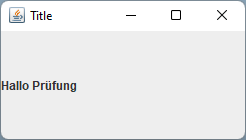
\includegraphics[width=0.3\columnwidth]{Images/swing1}
\end{center}
\begin{lstlisting}
import javax.swing.*;
	
public class HelloSwing {
	public static void main(String[] args) {
		JFrame frame = new JFrame("Title");
		frame.setSize(100, 30);
		
		frame.setDefaultCloseOperation(JFrame.EXIT_ON_CLOSE);
		
		JLabel label = new JLabel("Hallo Pruefung");
		frame.getContentPane().add(label);
		frame.pack(); // Minimal Groesse einnehmen
		frame.setVisible(true);
	}
}
\end{lstlisting}




\subsection{Event-Dispatch-Thread}
Jede Java Swing Applikation besitzt ein eigenen Event-Loop (Event-Dispatch-Thread EDT) welcher Events vom Native-Event-Loop an die Zuständige Komponente weiterleitet. Der Native-Event-Loop ist eine Zwischenstuffe um die Platform unabhängigkeit zum jeweliigen OS zu gewährlsiten. Events sind Ereignisse zB Tastendruck oder Mausklick, welche zum jeweiligen Program bzw. der entsprechenden Komponente weitergeleitet werden müssen. Mittels \textit{ActionListener} Interface können diese in der Komponenten registiert werden.

ActionListener werden häufig mit Lambdas oder Inner-Klassen implementiert.
\begin{lstlisting}
button1.addActionListener((e) -> {
		JFileChooser fc = new JFileChooser();
		fc.showOpenDialog(null);
	}
});

button1.addActionListener((e) -> {
		System.exit(0);
	}
});
\end{lstlisting}


\subsection{Layout-Manager}
\begin{tabular}{m{1cm} m{100px} m{4cm}}
	\textbf{Name} & \textbf{Beispiel} & \textbf{Eigenschaften} \\ \toprule
	Border & 	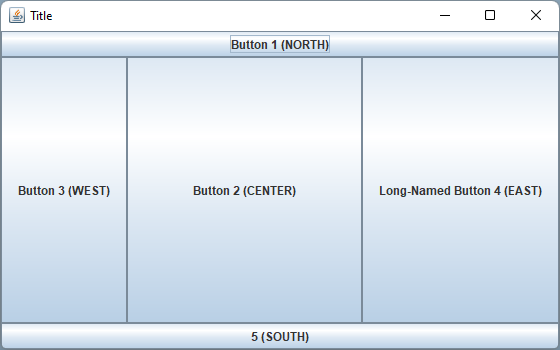
\includegraphics[width=100px]{Images/borderlayout} & \begin{itemize}[nosep]
		\item CENTER-Fläche wird maximiert
		\item Reihenfolge von add() irrelevant
		\item One Positionsangabe bei add(): CENTER
	\end{itemize} \\ \midrule
	Box & 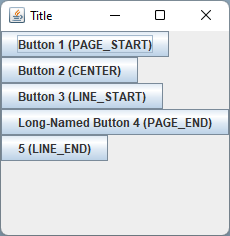
\includegraphics[width=100px]{Images/boxlayout} & \begin{itemize}[nosep]
		\item Komponenten werden in einer Reihe oder Spalte ausgegeben
		\item Alignment supported
		\item Vordert Maximale Grössen
	\end{itemize}  \\\midrule
	Card & 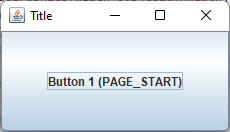
\includegraphics[width=100px]{Images/cardlayout} & \begin{itemize}[nosep]
		\item Überlagert Komponenten zB für TabbedPane oder JComboBox
	\end{itemize} \\\midrule
	Flow & 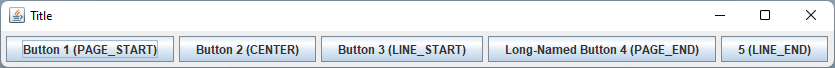
\includegraphics[width=100px]{Images/flowlayout} & \begin{itemize}[nosep]
		\item Komponenten werden in einer Riehe oder Spalte ausgegeben sofern Platz vorhanden
		\item Standard von JPanel
	\end{itemize} \\\midrule
	GridBag & 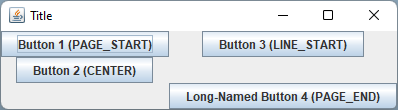
\includegraphics[width=100px]{Images/girdbag} & \begin{itemize}[nosep]
		\item Komponenten können mehrer Zellen besitzen
		\item Unterschiedliche Höhen und Breiten von Zellen
	\end{itemize} \\\midrule
	Grid & 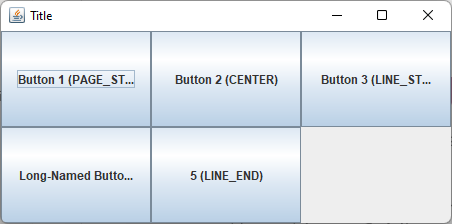
\includegraphics[width=100px]{Images/gridlayout} & \begin{itemize}[nosep]
		\item Macht Anzahl von Spalten und Zeilen gemäss Konstruktur
		\item Reihenfolge von add() bestimmt Anordnung
		\item Alle Zellen gleich gross
	\end{itemize} \\\midrule
		
\end{tabular}
	
\textbf{Beispiel}
\begin{lstlisting}
import javax.swing.*;
import java.awt.*;

public class MainProgram {
	public static void main(String[] args) {
		JFrame frame = new JFrame("Title");
		frame.setLayout(new BorderLayout());
		
		Container panel = frame.getContentPane();
		
		JButton button = new JButton("Button 1 (NORTH)");
		panel.add(button, BorderLayout.NORTH);
		
		button = new JButton("Button 2 (CENTER)");
		panel.add(button, FlowLayout.CENTER);
		
		button = new JButton("Button 3 (WEST)");
		panel.add(button, BorderLayout.WEST);
		
		button = new JButton("Long-Named Button 4 (EAST)");
		panel.add(button, BorderLayout.EAST);
		
		button = new JButton("5 (SOUTH)");
		panel.add(button, BorderLayout.SOUTH);
			
		frame.pack();
		frame.setVisible(true);
	}
}
\end{lstlisting}

	
\subsection{Swing Komponenten}
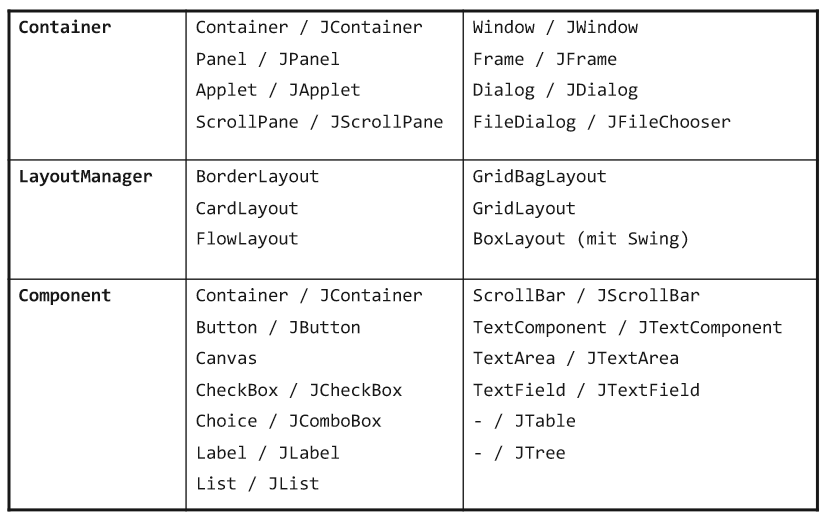
\includegraphics[width=\columnwidth]{Images/swing_komponenten}

	
